%---------------------------------------------------------------------------------------------------
% Einstellungen
% (gelten nur in Zusammenarbeit mit pdflatex)
%---------------------------------------------------------------------------------------------------
\documentclass[
  pagesize, % flexible Auswahl des Papierformats
  a4paper, % DIN A4
  oneside, % einseitiger Druck
  BCOR5mm, % Bindungskorrektur
  headsepline, % Strich unter der Kopfzeile
  11pt, % 11pt Schriftgröße
  parskip=half, % Europäischer Satz: Abstand zwischen Absätzen
  abstracton, % Spezielle Formatierung, die erlaubt, dass die Zusammenfassung vor dem Inhaltsverzeichnis steht
  %draft, % Es handelt sich um eine Vorabversion
  final, % Es handelt sich um die endgültige Version
  listof=totoc, % Tabellen- und Abbildungsverzeichnis im Inhaltsverzeichnis
  index=totoc, % Index im Inhaltsverzeichnis
  bibliography=totoc, % Literaturverzeichnis im Inhaltsverzeichnis
]{scrartcl}                                            % KOMA-Scriptklasse Report

%---------------------------------------------------------------------------------------------------
\usepackage[english,ngerman]{babel}                    % deutsche Trennmuster
\usepackage[T1]{fontenc}                               % EC-Schriften, Trennstellen nach Umlauten
\usepackage[utf8x]{inputenc}                          % direkte Umlauteingabe (ä statt "a)
                                                       % latin1/latin9 für unixoide Systeme
                                                       % (latin1 ist auch unter Win verwendbar)
                                                       % ansinew für Windows
                                                       % applemac Macs
                                                       % cp850 OS/2
\usepackage{times}                                     % Schriften Paket
\usepackage{array,ragged2e}                            % Wichtig für Abstandsformatierung

%---------------------------------------------------------------------------------------------------
\usepackage{cmbright}                                  % serifenlose Schrift als Standard
                                                       % + alle für TeX benötigten mathematischen
                                                       %   Schriften einschließlich der AMS-Symbole
\usepackage[scaled=.90]{helvet}                        % skalierte Helvetica als \sfdefault
\usepackage{courier}                                   % Courier als \ttdefault

%---------------------------------------------------------------------------------------------------
\usepackage[automark]{scrpage2}                        % Anpassung der Kopf- und Fußzeilen
\usepackage{xspace}                                    % Korrekter Leerraum nach Befehlsdefinitionen
\usepackage{setspace}                                  % Dieses Package brauchen wir für den anderthalbzeiligen Abstand.
\usepackage[numbers]{natbib}                           % Neuimplementierung des \cite-Kommandos
%\usepackage{bibgerm}                                  % Deutsche Bezeichnungen (deprecated)
\usepackage[german]{babelbib}                          % Deutsche Bezeichnungen
\usepackage[absolute, overlay]{textpos}                % placing boxes at absolute positions
\usepackage[final]{pdfpages}                           % include pages of external PDF documents
\usepackage{tabularx}                                  % Spaltenbreite bis zur Seitenbreite dehnen
\usepackage{makeidx}                                   % Paket zur Erstellung eines Stichwortverzeichnisses
\makeindex                                             % Automatische Erstellung des Stichwortverzeichnis
\usepackage[intoc,german,prefix]{nomencl}

\usepackage{listings}
\lstset{
  language=Matlab,
  basicstyle=\footnotesize,
  numbers=left,
  numberstyle=\tiny,
  captionpos=b}
\usepackage{caption}
\usepackage{subcaption}

% \usepackage{accents}

% \usepackage{footnote} % Ermöglicht Fußnoten in gleitenden Umgebungen
% \usepackage{capt-of} % Ermöglicht Beschriftungen beliebiger Objekte

\makenomenclature

%---------------------------------------------------------------------------------------------------
 \usepackage{graphicx}                                 % Zur Einbindung von PDF-Bildern
 \usepackage[colorlinks,                               % Einstellen und Laden des Hyperref-Pakets
  pdftex,
  bookmarks,
  bookmarksopen=false,
  bookmarksnumbered,
  citecolor=blue,
  linkcolor=blue,
  urlcolor=blue,
  filecolor=blue,
  linktocpage,
  pdfstartview=Fit,                                  % startet mit Ganzseitenanzeige
  pdfsubject={Hausarbeit im Rahmen der Vorlesung Modellierung technischer Systeme},
  pdftitle={Hausarbeit im Rahmen der Vorlesung Modellierung technischer Systeme},
  pdfauthor={Andreas Krohn}]{hyperref}
% \pdfcompresslevel=9
%\usepackage{wrapfig}

%---------------------------------------------------------------------------------------------------
% Inhaltsverzeichnis und Abschnittnummerierung
%---------------------------------------------------------------------------------------------------
\setcounter{secnumdepth}{2}   % Ich habe recht kurze Kapitel. Die sollen nicht durchnummeriert sein.
\setcounter{tocdepth}{2}

%---------------------------------------------------------------------------------------------------
% Abbildungsverzeichnis
%---------------------------------------------------------------------------------------------------
\graphicspath{{graphics/}}

%---------------------------------------------------------------------------------------------------
% Kopf- und Fußzeilen
%---------------------------------------------------------------------------------------------------
\pagestyle{scrheadings}
\clearscrheadings
\clearscrplain
\clearscrheadfoot
\ohead{\pagemark}
\ihead{\headmark}

%---------------------------------------------------------------------------------------------------
% Neue Befehle
%---------------------------------------------------------------------------------------------------
%---------------------------------------------------------------------------------------------------
% Neue Befehle
%---------------------------------------------------------------------------------------------------

%---------------------------------------------------------------------------------------------------
% Umbenennen des Symbolverzeichnisses
%---------------------------------------------------------------------------------------------------
\renewcommand{\nomname}{Glossar}				% Das Symbolverzeichnis heisst nun "Glossar"
\renewcommand{\nomlabel}[1]{						% Die zu erklärenden Begriffe sind nun fett hervorgehoben
	\hfil \textbf{#1} \hfil
}

%---------------------------------------------------------------------------------------------------
% Ein paar ganz nützliche Befehle von Lars Mählmann
%---------------------------------------------------------------------------------------------------
%für Kommentare
\newcommand{\colb}{\color{green}}
\newcommand{\colbl}{\color{black}}

%---------------------------------------------------------------------------------------------------
% Befehle zum Erstellen des Index
% \addIndexEntry{Eintrag in den Index}
% \addSubIndexEntry{Eintrag in den Index}{Eintrag des übergeordneten Eintrags}
%---------------------------------------------------------------------------------------------------
\newcommand{\addIndexEntry}[1]{#1\index{#1}}
\newcommand{\addSubIndexEntry}[2]{#1\index{#2!#1}}

%---------------------------------------------------------------------------------------------------
% LaTeX in eigenem Font
%---------------------------------------------------------------------------------------------------
\newcommand{\myLatex}{
	{\rmfamily\LaTeX\xspace}
}

%---------------------------------------------------------------------------------------------------
% Befehl zum Erstellen und Hervorheben eines Zitats
% Parameter:
% 1. Zitat
% 2. Author
% 3. Quelle
%---------------------------------------------------------------------------------------------------
\newcommand{\myCitation}[3]{
	\begin{flushright}
	\begin{minipage}{.4\linewidth}
		\footnotesize\rmfamily\itshape
		#1 \\
		\RaggedLeft #2 \\
		#3
	\end{minipage}
	\end{flushright}
	\nobreakspace
}

%---------------------------------------------------------------------------------------------------
% Erstellung von Deckblatt (Seite 1) und Titelblatt (Seite 2)
%---------------------------------------------------------------------------------------------------
\newcommand{\createCoverAndTitlePage}[8]{
	\createCover{#1}{#2}{#3}
	\createTitlePage{#1}{#2}{#3}{#4}{#5}{#6}{#7}{#8}
}

%---------------------------------------------------------------------------------------------------
% Erstellung von Deckblatt (Seite 1)
% Anwendung:
% \createCover{Art der Arbeit}{Autor}{Titel}
%---------------------------------------------------------------------------------------------------
\newcommand{\createCover}[3]{
	\thispagestyle{empty}
	\begin{titlepage}

	\setlength{\TPHorizModule}{1mm}
	\setlength{\TPVertModule}{1mm}
	\textblockorigin{0mm}{0mm} % start everything near the top-left corner

	% Art der Arbeit
	\begin{textblock}{111}(83,115)
		\begin{minipage}[c][1,78cm][c]{11,09cm}
  		\fontsize{22pt}{20pt}
  		\selectfont
  		\begin{center}
  		#1
  		\end{center}
		\end{minipage}
	\end{textblock}

	% Name & Titel
	\begin{textblock}{111}(83,131)
		\begin{minipage}[c][4,81cm][t]{11,09cm}
		\linespread{1.2}
    \fontsize{16pt}{14pt}
    \selectfont
    \begin{center}
    #2 \\ \medskip
    #3
    \end{center}
    \end{minipage}
	\end{textblock}
	% Infos zur Arbeit und zum Fachbereich
	\begin{textblock}{186}(22,264)
  	\begin{minipage}[t][5,72cm][l]{17,57cm}
    	\fontsize{12pt}{12pt}
    	\selectfont
			{\em Fakultät Technik und Informatik \hfill Faculty of Engineering and Computer Science}\\
			{\em Department Informatik \hfill Department of Computer Science}
  	\end{minipage}
	\end{textblock}
	\newpage
	\end{titlepage}
%---------------------------------------------------------------------------------------------------
% Wichtig! Entsprechendes Auskommentieren!
%---------------------------------------------------------------------------------------------------
	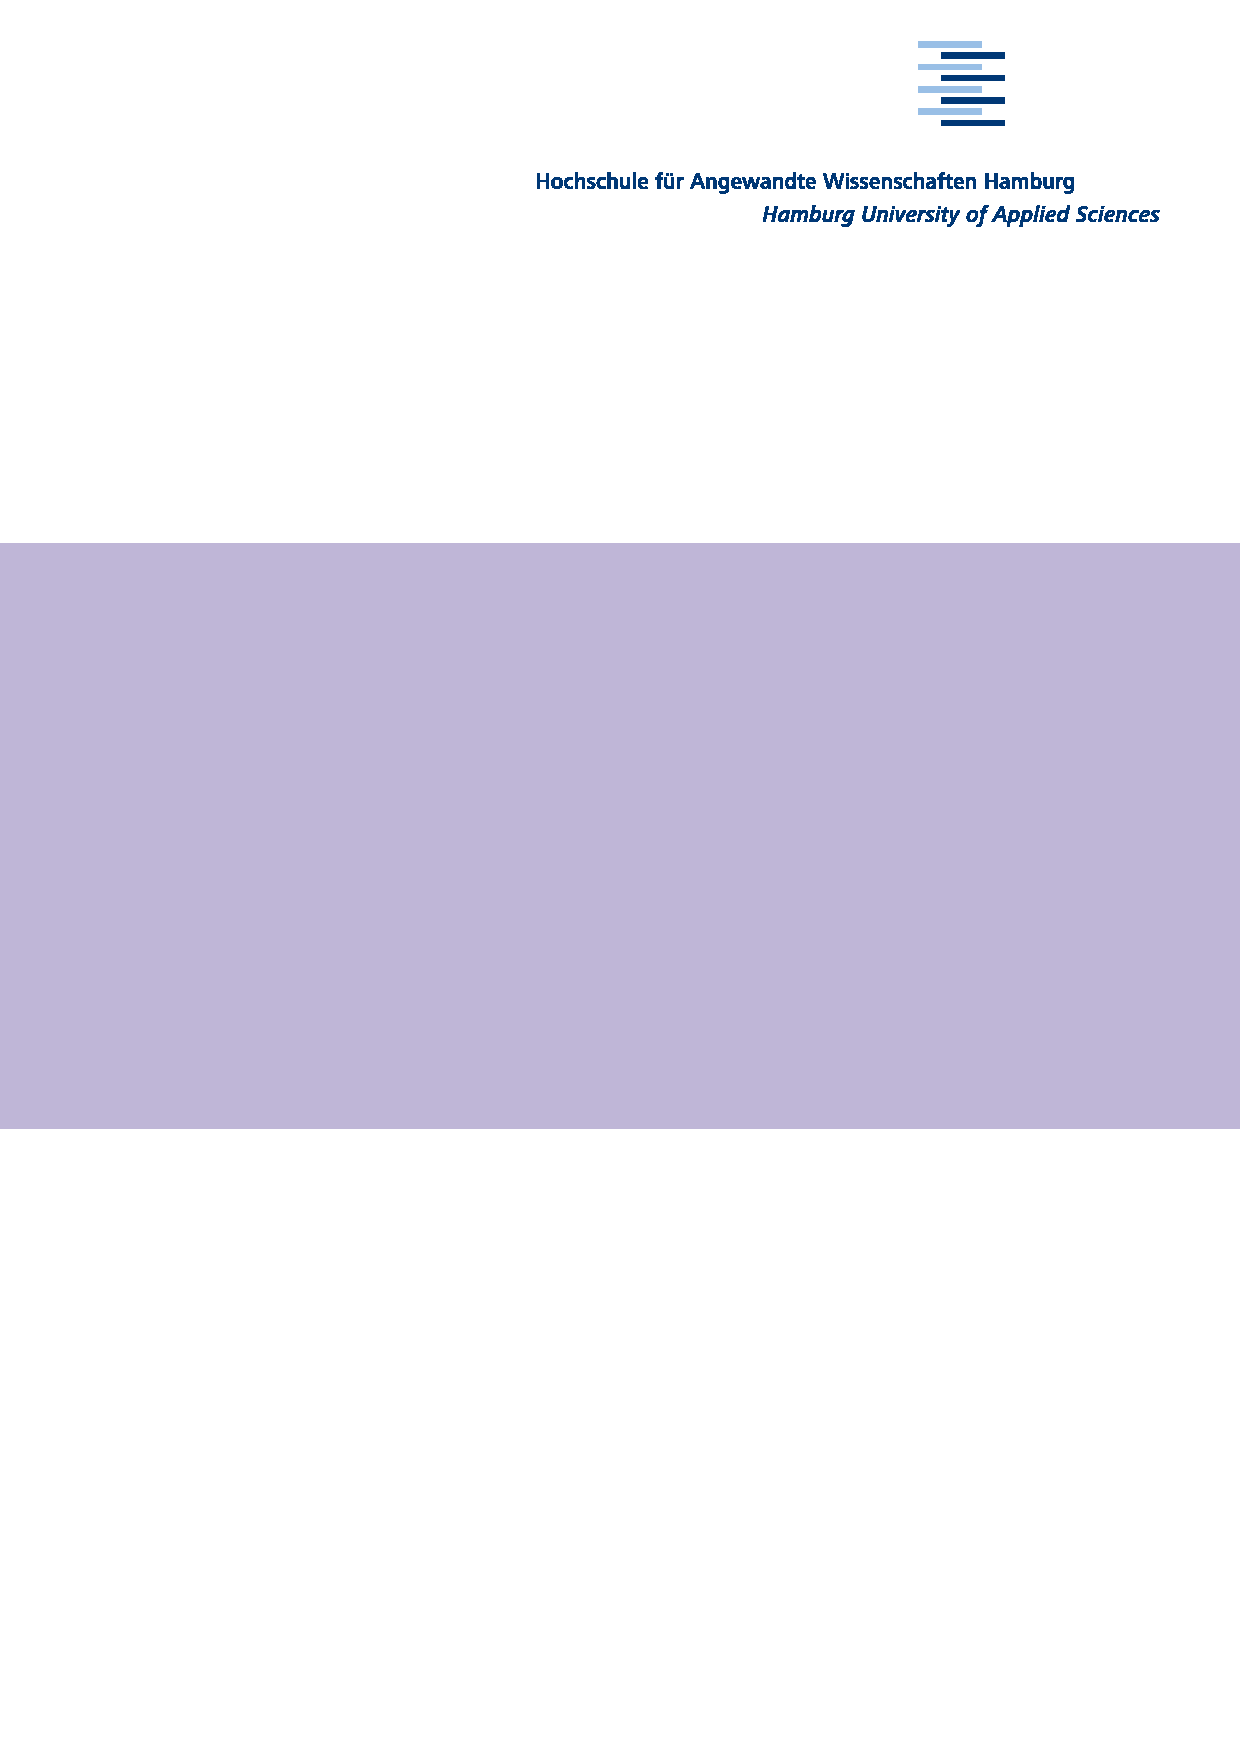
\includepdf{pdf/titel}           				% zum Ausdruck auf blanko Papier
  %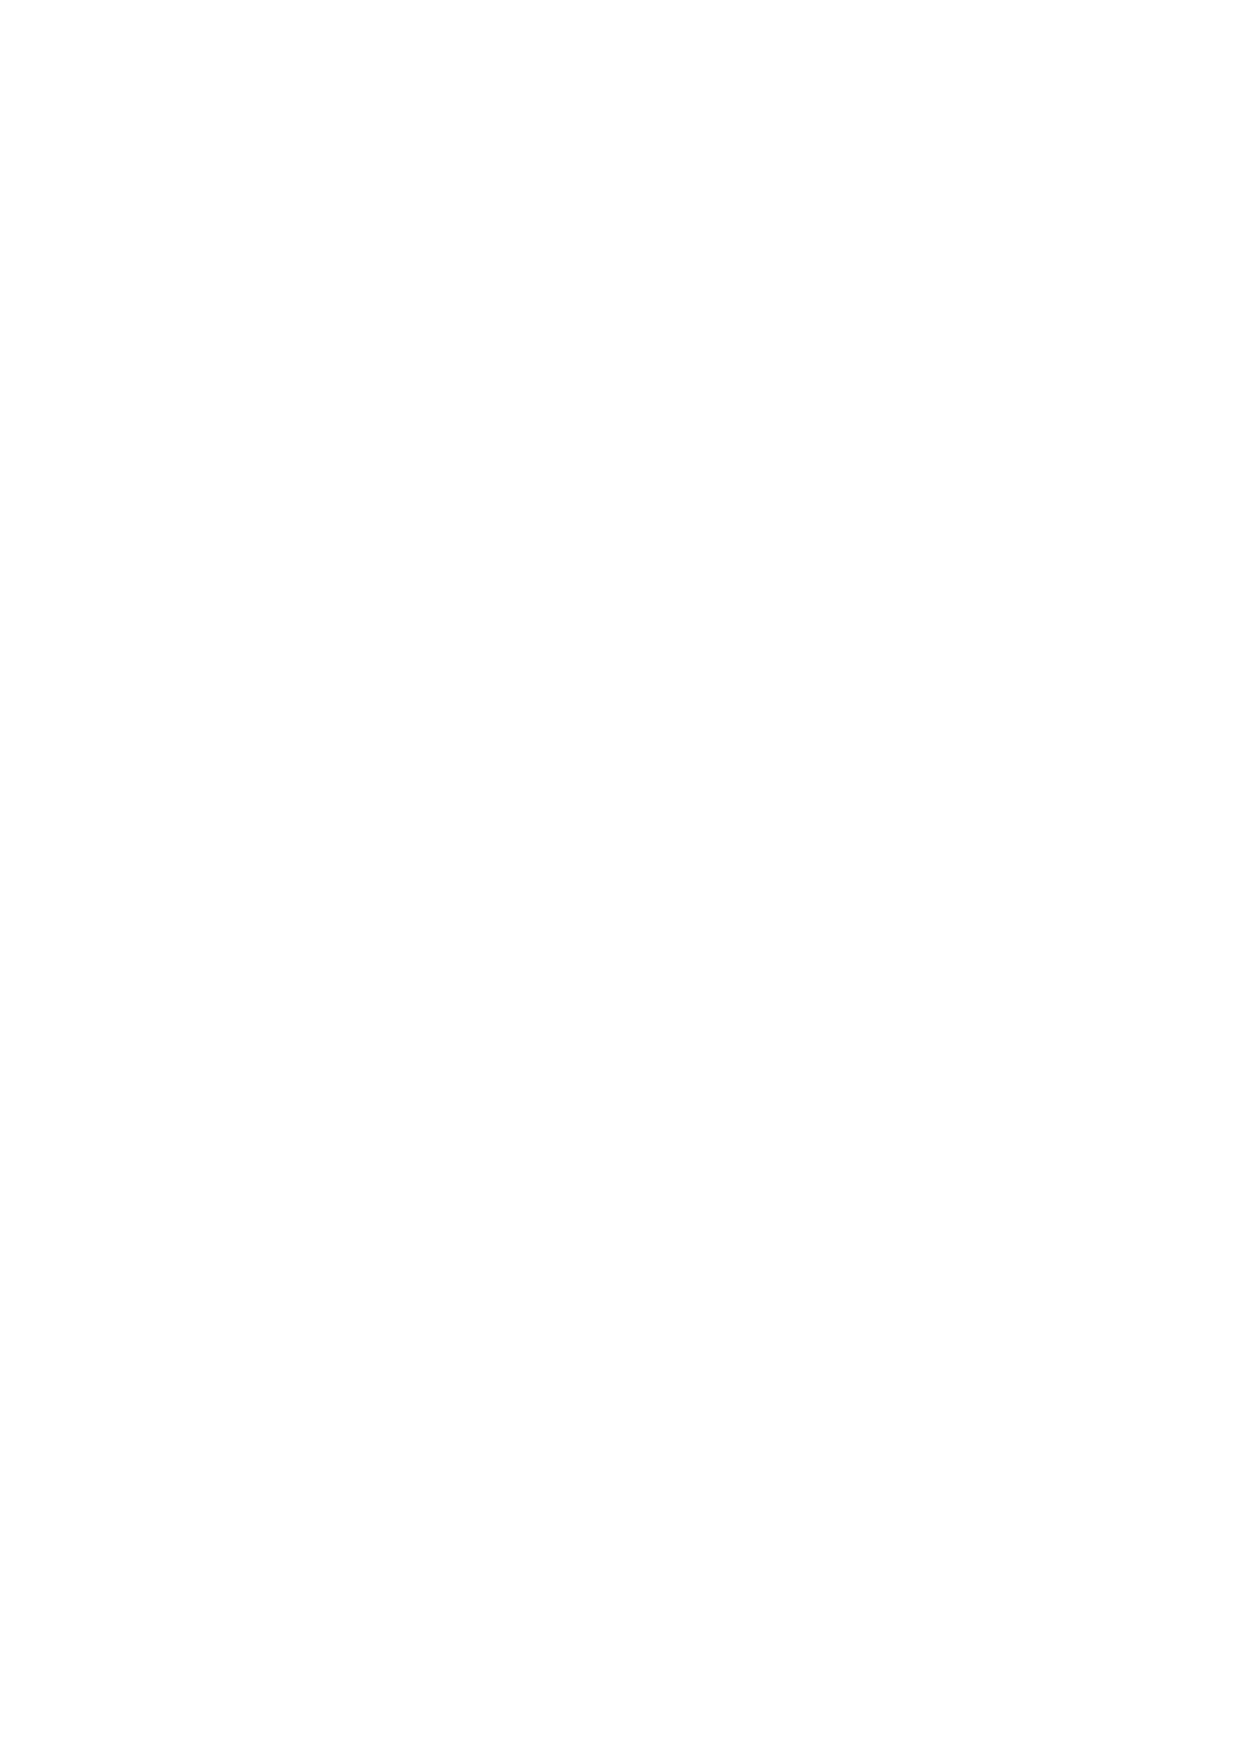
\includepdf{pdf/titel_leer}           	% zum Ausdruck auf die Pappe
}

%---------------------------------------------------------------------------------------------------
% Erstellung von Titelblatt (Seite 2)
% Anwendung:
% \createTitlePage{Art der Arbeit}{Author}{Titel}{Studiengang}{Erstprüfer}{Zweitprüfer}
%---------------------------------------------------------------------------------------------------
\newcommand{\createTitlePage}[7]{
	\thispagestyle{empty}

	\setlength{\TPHorizModule}{1mm}
	\setlength{\TPVertModule}{\TPHorizModule}
	\textblockorigin{0mm}{0mm} % start everything near the top-left corner

	% Name & Titel
	\begin{textblock}{130}(40,63)
		\begin{minipage}[c][5,9cm][t]{13cm}
			\begin{center}
			\linespread{1.2}
			\fontsize{18pt}{18pt}
  		\selectfont
  		#2 \\ \medskip
  		\fontsize{16pt}{16pt}
  		#3
  		\end{center}
		\end{minipage}
	\end{textblock}

	% Infos zur Arbeit und zum Fachbereich
	\begin{textblock}{126}(32,214)
  	\begin{minipage}[t][5,72cm][l]{12,57cm}
    	\fontsize{12pt}{12pt}
    	\selectfont
    	#1 eingereicht im Rahmen der #1prüfung\\
    	im Studiengang #4\\
			am Department Informatik\\
			der Fakultät Technik und Informatik\\
			der Hochschule für Angewandte Wissenschaften Hamburg\\
			\\\
			\\\
			Betreuender Prüfer : #5\\
			Zweitgutachter : #6\\
			\\\
			Abgegeben am \today
  	\end{minipage}
	\end{textblock}
	\	% WICHTIG! Damit wird nach dem Titelblatt eine neue Seite angefangen! Sonst werden Titelblatt &
  	% Danksagung auf eine Seite gedruckt!
}

%---------------------------------------------------------------------------------------------------
% Versicherung über Selbstständigkeit
%---------------------------------------------------------------------------------------------------
\newcommand{\asurency}{
	\chapter*{Versicherung über Selbstständigkeit}
	\vfill
	Hiermit versichere ich, dass ich die vorliegende Arbeit im Sinne der Prü\-fungs\-ord\-nung nach \S 24(5) 		ohne fremde Hilfe selbstständig verfasst und nur die angegebenen Hilfsmittel benutzt habe.
	\vfill
	\begin{tabularx}{\linewidth}{X l X}
	Hamburg, \today	& \qquad \qquad \qquad	& \\
	\cline{1-1}
	\cline{3-3}
	Ort, Datum	& \qquad \qquad \qquad	& Unterschrift \\
	\end{tabularx}
	\vfill
	\vfill
	\vfill
}

%---------------------------------------------------------------------------------------------------
% Fügt ein Wort dem Index zu
%---------------------------------------------------------------------------------------------------
\newcommand{\toIndex}[1]{#1\index{#1}}

%---------------------------------------------------------------------------------------------------
% Dient zum Eintragen folgender Dinge in die Zusammenfassung (Abstract):
%	- Thema
% - Stichworte
% - Kurzfassung
% Benutzung wie folgt:
% \abstractentry{Titel}{Text}
%---------------------------------------------------------------------------------------------------
\newcommand{\abstractentry}[2]{
	\textbf{\large#1}\\
	\nobreakspace
	\begin{tabular}{lp{142mm}}
		\hspace*{7mm} & #2 \\
	\end{tabular}
	\vfill
}

%---------------------------------------------------------------------------------------------------
% Erstellt eine Defintion
% Anwendung: \definition{Die Definition}
%---------------------------------------------------------------------------------------------------
\newcommand{\definition}[1]{
\begin{tabular}[ht]{lp{135mm}}
	\textbf{Def.:} & #1 \\
\end{tabular}
}

%---------------------------------------------------------------------------------------------------
% Erstellt eine Widmung
% Anwendung: \dedication{Wem ist das Schriftstück gewidmet}
%---------------------------------------------------------------------------------------------------
\newcommand{\createDedication}[1]{
	\newpage
	\thispagestyle{empty}
	\begin{tabular}{lp{60mm}}
		\hspace*{100mm} & \itshape\rmfamily#1 \\
	\end{tabular}
	\vfill
}

%---------------------------------------------------------------------------------------------------
% Häufig verwendete Namen mit Literaturverweis und Indexeintrag
%--------------------------------------------------------------------------------------------------
\newcommand{\butrynowski}{Christian Butrynowski\index{Butrynowski, Christian} \citep{Butrynowski:2005}\xspace}
\newcommand{\luepke}{André Lüpke\index{Lüpke, André}\citep{Luepke:2004}\xspace}
\newcommand{\bresch}{Marco Bresch\index{Bresch, Marco} \citep{Bresch:2004}\xspace}


%---------------------------------------------------------------------------------------------------
% Die folgenden Befehle wurden aus der Vorlage von Michael Knop übernommen
%--------------------------------------------------------------------------------------------------
%---------------------------------------------------------------------------------------------------
% Ident
%---------------------------------------------------------------------------------------------------
\newcommand{\ident}[1]{                             % ein Parameter
	\small\ttfamily#1\sffamily\normalsize
}

%---------------------------------------------------------------------------------------------------
% Kürzel
%---------------------------------------------------------------------------------------------------
% Hier sind Makros definiert, die die Eingabe erleichtern sollen. Für korrekte Abstände zwischen
% "z.B." sorgt also ein "z.\,B." (LaTeX-Befehl für kleineren Abstand)
% Schneller schreibt sich das durch das Makro "\zB":

% \newcommand{\zB}{z.\,B.\ }

% Hier ist der Rest aber mit dem Paket xspace verwirklicht. Damit kann
% man bei Bedarf den Abstand mit "\hspace" exakt eingeben. Dann zeigt
% LaTeX keine Toleranz bei den Abkürzungen und macht eben exakt das
% untenstehende.

%\renewcommand{\entryname}{K\"urzel}
%\renewcommand{\descriptionname}{Beschreibung}

\newcommand{\vgl}{vgl.\@\xspace}
\newcommand{\abb}{Abb.\@\xspace}
\newcommand{\zB}{z.\nolinebreak[4]\hspace{0.125em}\nolinebreak[4]B.\@\xspace}
\newcommand{\bzw}{bzw.\@\xspace}
\newcommand{\dahe}{d.\nolinebreak[4]\hspace{0.125em}h.\nolinebreak[4]\@\xspace}
\newcommand{\etc}{etc.\@\xspace}
\newcommand{\bzgl}{bzgl.\@\xspace}
\newcommand{\so}{s.\nolinebreak[4]\hspace{0.125em}\nolinebreak[4]o.\@\xspace}
\newcommand{\iA}{i.\nolinebreak[4]\hspace{0.125em}\nolinebreak[4]A.\@\xspace}
\newcommand{\sa}{s.\nolinebreak[4]\hspace{0.125em}\nolinebreak[4]a.\@\xspace}
\newcommand{\su}{s.\nolinebreak[4]\hspace{0.125em}\nolinebreak[4]u.\@\xspace}
\newcommand{\ua}{u.\nolinebreak[4]\hspace{0.125em}\nolinebreak[4]a.\@\xspace}
\newcommand{\og}{o.\nolinebreak[4]\hspace{0.125em}\nolinebreak[4]g.\@\xspace}

\newcommand{\HAW}{Hochschule für Angewandte Wissenschaften Hamburg\xspace}
\newcommand{\GNU}{GNU\xspace}
\newcommand{\GPL}{\GNU Public License\xspace}

\newcommand{\ACM}{ACM\xspace}
\newcommand{\PDA}{PDA\xspace}


%---------------------------------------------------------------------------------------------------
% Trennung
%---------------------------------------------------------------------------------------------------
%---------------------------------------------------------------------------------------------------
% Trennung
% Hier können alle Wörtertrennungen definiert werden. Die nachfolgenden dienen als Beispiel
% und wurden aus der Vorlage von Michael Knop übernommen.
%---------------------------------------------------------------------------------------------------
\hyphenation{Web-ap-pli-ka-tion Web-ap-pli-ka-tio-nen Web-an-wen-dung Web-an-wen-dung-en My-SQL Kon-text-in-for-ma-ti-onen}

%---------------------------------------------------------------------------------------------------
% Anpassung der Parameter, die TeX bei der Berechnung der Zeilenumbrüche verwendet:
%---------------------------------------------------------------------------------------------------
\tolerance 1414
\hbadness 1414
\emergencystretch 1.5em
\hfuzz 0.3pt
\widowpenalty=10000
\vfuzz \hfuzz
\raggedbottom
 % Die stilistischen Parameter

\date{\today}
%---------------------------------------------------------------------------------------------------
% Anfang des Schriftstücks
%---------------------------------------------------------------------------------------------------
\begin{document}

%---------------------------------------------------------------------------------------------------
% Erstellen des Deck- und des Titelblatts
%---------------------------------------------------------------------------------------------------
\createCover{Modellierung eines Sprungs aus großer Höhe} % Art der Arbeit
{Andreas Krohn} % Author
{Hausarbeit im Rahmen der Vorlesung Modellierung technischer Systeme\\
WS2012/13 - 09.01.2012} % Title

%---------------------------------------------------------------------------------------------------
% Zusammenfassung}
%---------------------------------------------------------------------------------------------------
% %---------------------------------------------------------------------------------------------------
% Zusammenfassung
%---------------------------------------------------------------------------------------------------
\newpage
\thispagestyle{empty}
\subsection*{Martin Mustermann}
\abstractentry{Thema der Bachelorarbeit}{Mein Titel der Arbeit: Sollte kurz und interessant klingen und nicht die gesamte Aufgabenstellung und Abgrenzungen beinhalten.}
\abstractentry{Stichworte}{...die wichtigsten Stichwörter}
\abstractentry{Kurzzusammenfassung}{
In dieser Arbeit wurde....
}

\selectlanguage{english}
\subsection*{Martin Mustermann}
\abstractentry{Title of the paper}{My title of the paper: Should sound short and interesting and should not contain the complete type of problem and delimitations.}
\abstractentry{Keywords}{...the most important keywords}
\abstractentry{Abstract}{
In this paper...
}
\selectlanguage{ngerman}


%---------------------------------------------------------------------------------------------------
% Verzeichnisse
%---------------------------------------------------------------------------------------------------
\tableofcontents % Inhaltsverzeichnis
% \listoftables % Tabellenverzeichnis
% \listoffigures % Abbildungsverzeichnis

%---------------------------------------------------------------------------------------------------
% Einführung
%---------------------------------------------------------------------------------------------------
\newpage

\section{Einführung}

Die Raumfahrt ist der Versuch der Beherrschung komplexer Technologie.
Dennoch geschehen Unfälle, die gerade in der Start- und Landephase für Gerät und Astronauten katastrophal enden.
Die letzten Unglücke mit umgekommenen Personen waren die Space Shuttles Columbia im Jahre 2003 und Challenger im Jahre 1986.
Im Falle der Challenger gibt es Stimmen, die behaupten, dass die Crew mit einem Rettungssystem hätte überleben können.
Ein Rettungszenario wäre Ausstieg, freier Fall bis in dichtere Atmosphärenschichten und Landung mittels Fallschirm.
Gesteigertes Interesse an der Sicherheit gibt es angesichts der zunehmenden privaten Raumfahrt und der Vision Privatpersonen als Touristen in den Orbit zu transportieren.

\begin{figure}[h]
  \centering
  \begin{subfigure}[b]{0.25\textwidth}
    \centering
    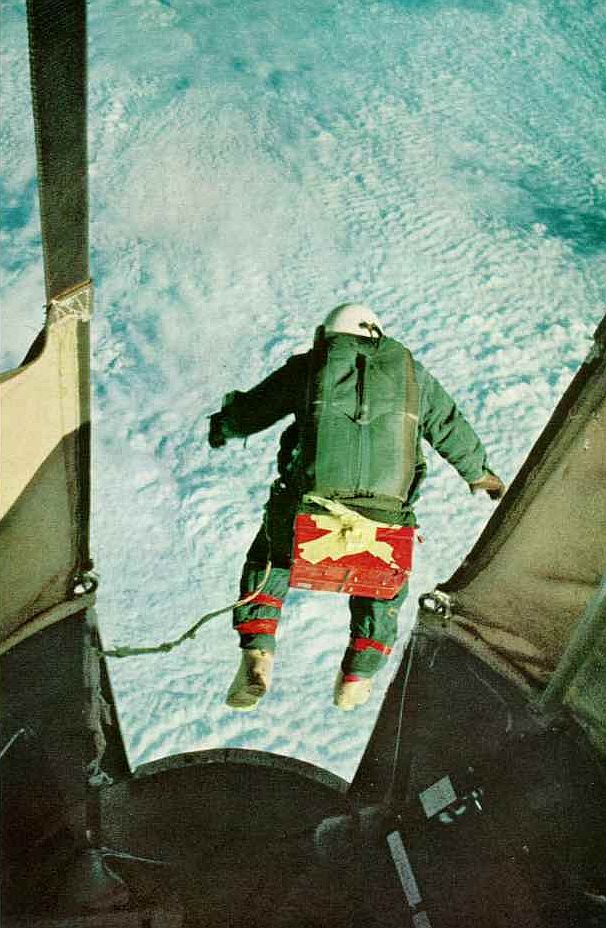
\includegraphics[width=1\textwidth]{excelsior-III-d}
    \caption{Joseph Kittinger\protect\footnotemark}
    \label{fig:excelsior-III-d}
  \end{subfigure}
  ~
  \begin{subfigure}[b]{0.25\textwidth}
    \centering
    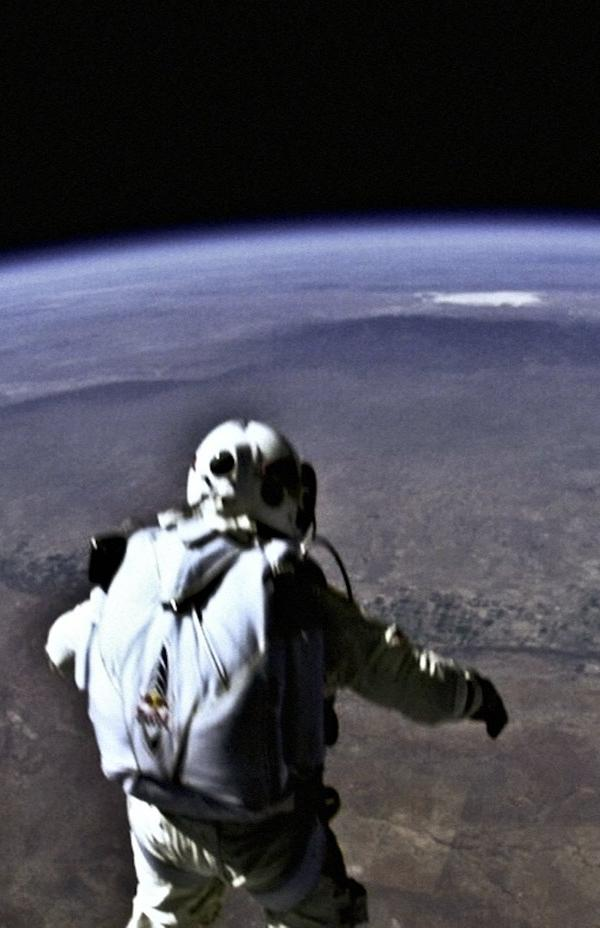
\includegraphics[width=1\textwidth]{baumgartner}
    \caption{Felix Baumgartner\protect\footnotemark}
    \label{fig:baumgartner}
  \end{subfigure}
  \caption{Absprung}
\end{figure}
\footnotetext[1]{Bildquelle: \url{http://stratocat.com.ar/fichas-e/1960/HMN-19600816.htm}}
\footnotetext{Bildquelle: \url{http://www.redbullstratos.com/gallery/}}

Der Fallschirmsprung aus der Stratosphäre wurde unter anderem im Rahmen des Projekts \emph{Excelsior}~\cite{af.mil:excelsior} bereits in den Jahren 1959 und 1960 getestet.
Hierbei lag der Fokus allerdings mehr auf Rettungstrategien für die Besatzungen hoch fliegender Jets.
Grundlegend wurde hierbei bereits die Machbarkeit von Fallschirmsprüngen aus einer Höhe von $30km$ bewiesen.
Der damalige Springer Joseph Kittinger führte drei Sprünge durch.
Es gibt umstrittene Behauptungen, dass er beim letzten Sprung aus $31.333m$ Höhe die Schallmauer durchbrochen hat.
Seit 2009 ist Kittinger am Red Bull Projekt beteiligt und half beratend beim Brechen seiner eigenen Rekorde mit.

Der Getränkehersteller Red Bull hat in den letzten Jahren ein Projekt finanziert, dass in den medienwirksamen Sprung des Österreichers Felix Baumgartners am 14.10.2012 mündete~\cite{rbstratos}.
Er stieg in einer Kapsel mittels Heliumballon in eine Höhe von $39.045m$ auf (geplant waren mindestens $35.576m$) und sprang.
Der Sprung stellte neue Rekorde auf, zum Beispiel das diesmal anerkannte Durchbrechen der Schallmauer ohne Flugzeug im freien Fall~\cite{fai:record}.
Weiterhin wurde erneut der Beweis erbracht, dass der Sprung aus derartigen Höhen möglich und dieser Weg als Rettungstrategie denkbar ist und medizinische Daten gesammelt.

Um die Frage zu klären, welche Absprunghöhe nötig ist, um die Schallmauer zu durchbrechen, soll das Experiment simuliert werden.
Dabei soll untersucht werden, wie der Sprung aus unterschiedlichen Höhen verlaufen wäre und welche Faktoren dabei eine Rolle spielen.
Weiterhin wird gezeigt, welche Geschwindigkeit bei einem ungebremsten Fall auf Höhe der Erdoberfläche erreicht wird.

In Kapitel \ref{sec:modellierung} wird auf die Modellierung des Sprungs eingegangen, wirkende Kräfte und gewählte Parameter beschrieben. Das Kapitel \ref{sec:simulation} beschreibt den Aufbau der Simulation, Kapitel \ref{sec:auswertung} wertet die Ergebnisse aus.
% Das Überschreiten vermeintlicher Grenzen gepaart mit Neugier (und die Aussicht auf Ruhm) sind ein starker Antrieb des Menschen.
% Luft- und Raumfahrt sind eine Frucht dieser Motive.
% Trotz aller Vorkehrungen werden hierbei Risiken eingegangen.
% Im Falle der Raumfahrt zwar nur von einigen wenigen Menschen, trotzdem gibt es Bestrebungen hier die Sicherheit zu erhöhen.
% Red Bull hat hierzu medienwirksam ein Experiment finanziert:
% Der Sprung des österreichischen Felix Baumgartners aus einer geplanten Höhe von 36.576m.
% Neben der Werbewirkung und dem Aufstellen neuer Rekorde sollten dabei medizinische Daten gesammelt und die Machbarkeit eines Notausstiegs von Astronauten in großer Höhe und der Rückkehr im freien Fall getestet werden.

%---------------------------------------------------------------------------------------------------
% Modellierung
%---------------------------------------------------------------------------------------------------
\section{Modellierung}\label{sec:modellierung}

Das Experiment besteht grob aus drei Phasen:
\begin{itemize}
  \item Aufstieg im Ballon
  \item Absprung und freier Fall
  \item Gebremster Fall am Fallschirm und Landung
\end{itemize}
Der Aufstieg wird im Rahmen dieser Arbeit nicht weiter betrachtet.
Interessanter ist der Fall - vor allem der ungebremste Abschnitt von Absprung bis zum Öffnen des Fallschirms.
Um dies zu simulieren, müssen relevante Kräfte und Größen berücksichtigt werden. %identifiziert und modelliert werden.

Seitenwinde und mögliche Rotation werden nicht modelliert.
Als Masse für Springer und Ausrüstung werden $140kg$ angeommen.
Auf den Springer und seine Ausrüstung wirken lediglich zwei Kräfte:
\begin{description}
  \item[$F_g$] Zur Erde hin wirkt die Gravitation.
  \item[$F_w$] Bremsend wirkt der Luftwiderstand.%, der sich bei Öffnen des Fallschirms massiv erhöht.
\end{description}

Die ausschlaggebenden Größen werden im Folgenden beschrieben.

\subsection{Gravitation}
Die Gravitation wirkt zwischen dem Springer und der Erde.
Allgemein wird hier das newtonsches Gravitationsgesetz angewendet.
\begin{equation}
F_g=G \frac{m_1 m_2}{r^2}
\end{equation}
Dabei ist $G$ die Gravitationskonstante $66.7384\times 10^{-12} \frac{m^3}{kg\ s^2}$, $m_1$ und $m_2$ die beteiligten Massen und $r$ deren Abstand.
Bis auf $r$ (der Springer bewegt sich ja auf die Erde zu) sind hier alle Größen konstant.
$r$ ist dabei gleich dem Radius der Erde $r_E$ plus der Höhe des Springers $h$ \vgl Abb.~\ref{fig:gravitation}.
\begin{figure}[h]
  \centering
  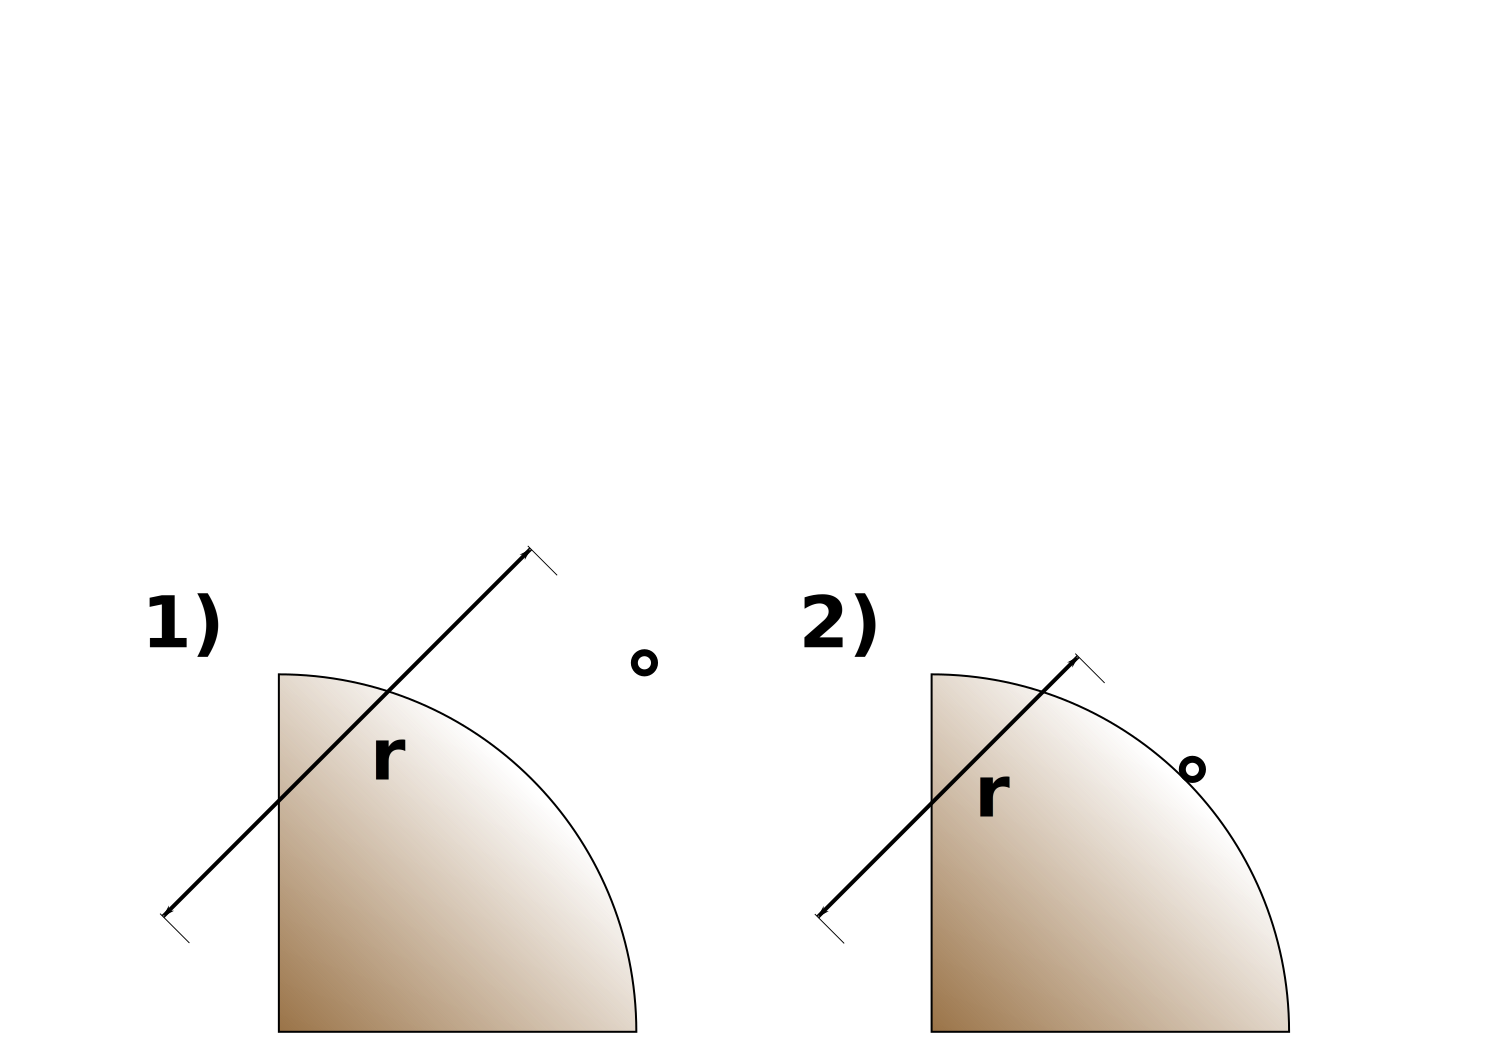
\includegraphics[width=0.5\textwidth]{gravitation}
  \caption{$r$ bei 1) Absprung und 2) Landung}
  \label{fig:gravitation}
\end{figure}

Als Erdradius wird der Äquatorradius $r_E=6 378 137m$ angenommen, als Masse des Springers $m_S=140kg$, als Masse der Erde $m_E=5.9736\times 10^{24}kg$.
Die Kraft, die auf den Springer auf Erdniveau herrscht beträgt
\begin{eqnarray}
F_{g_0} &=& 66.7384\cdot 10^{-12} \frac{140\cdot 5.9736\cdot 10^{24}}{6 378 137^2} \\
 &=& 1372 N \nonumber
\end{eqnarray}
Die Challenger zerbrach in $15km$ Höhe, der Sprung Baumgartners erfolgte aus knapp $40km$.
Um den Effekt der Höhenänderung deutlich zu zeigen wird als zweiter Wert die Gravitationskraft in $40km$ Höhe berechnet.
\begin{eqnarray}
F_{g_1} &=& 66.7384\cdot 10^{-12} \frac{140\cdot 5.9736\cdot 10^{24}}{\left(6 378 137 + 40 000\right)^2} \\
 &=& 1354.9 N \nonumber
\end{eqnarray}
Die Gravitationskraft nimmt in Absprunghöhe gegenüber der auf Erdniveau herrschenden um knapp $2\%$ ab.
Die Veränderung ist nicht groß, wird aber in der Simulation berücksichtigt.

\subsection{Luftwiderstand}
Der Fall des Springers wird durch den von der Atmosphäre verursachten Luftwiderstand gebremst.
Zur Berechnung dieser Kraft wird die Formel für den Strömungswiderstand verwendet.
\begin{equation}
F_w=\frac{1}{2}pv^2c_wA
\end{equation}
In die Berechnung der Kraft gehen die aktuelle Geschwindigkeit $v$, der Strömungswiderstandskoeffizient $c_w$, die angeströmte Fläche $A$ und die Dichte des umgebenden Mediums $p$ ein.
Die Geschwindigkeit ist das Integral der Beschleunigung, ergibt sich also zu jedem Zeitpunkt aus der Simulation.
Die Wahl von $p$, $c_w$ und $A$ werden im Folgenden beschrieben.
%Die Widerstandsfläche ändert sich bei Öffnung des Fallschirms.
%Weiterhin steigt die Widerstandsfläche in der Nähe der dichte- und temperaturabhängigen Schallgeschwindigkeit an.

\paragraph{Atmosphärenmodell}
Mit steigender Höhe nimmt der Luftdruck ab, da die darüberliegende Gassäule kürzer und somit leichter wird.
Auch die Temperatur ist höhenabhängig.
Zunächst ist die Temperatur der Erdoberfläche der ausschlaggebende Faktor.
Mit zunehmender Höhe nimmt dieser Einfluss ab und die Temperatur sinkt.
Ab einer bestimmten Höhe nimmt die Temperatur wieder zu, da ein immer geringerer Anteil der Einstrahlung von darüberliegenden Atmosphärenschichten blockiert wird.
Die Höhe, ab der die Temperatur wieder steigt ist von vielen Faktoren wie zum Beispiel der Tages- und Jahreszeit abhängig.
Nach einiger Beschäftigung mit Meteorologie, der Schichtung der Atmosphäre, Höhenformeln, virtueller Temperatur usw.~\cite{met:einfuehrung, met:umwelt}, wurde für die Simulation auf die eigene Umsetzung eines Atmosphärenmodells verzichtet.

Für die Simulation von Dichte und Temperatur wird das empirische NRLMSISE-00-Modell~\cite{nrlmsise00:goddardspaceflightcenter} verwendet, das in Matlab und Simulink als Funktion und Block zur Verfügung steht~\cite{matlab:mrlmsise-00}.
Es liefert abhängig von den Parametern Datum, Uhrzeit und geographische Position in einem Höhenbereich von $0$ bis $100km$ Werte für Dichte und Temperatur.
Für die Simulation wird lediglich die Höhe variiert und die anderen Parameter mit Ort und Zeit des Baumgartner-Experiments konstant vorbelegt.
Dichte und Temperatur stehen also jeweils als Funktion der Höhe zur Verfügung.

\paragraph{Strömungswiderstandskoeffizient und -fläche}
Der $c_w$-Wert eines Menschen liegt laut Zatsiorsky~\cite[88]{humankinetics} lageabhängig in einer Spanne von $0.35$ bis $1.36$.
Die höheren Werte gelten dabei für Lagen quer zum Luftstrom, das niedere Ende des Spektrums für Lagen längs zum Luftstrom.
Auch die angeströmte Fläche $A$ ist von der Richtung des Luftstroms abhängig.
Da Felix Baumgartner kurz nach dem Absprung in Rotation geriet und somit nicht kontinuierlich kopfüber längs zum Luftstrom fiel, werden für die Simulation die Werte $c_w=1.3$ und $A=0.8$ geschätzt, was in etwa dem in \cite{redbulletin:stratosspecialde} auf Seite 59 genannten Wert $c_w\cdot A=1.07$ entspricht.

\subsection{Gesamtmodell}

\begin{figure}[h]
  \centering
  \includegraphics[width=0.5\textwidth]{forces}
  \caption{Wirkende Kräfte}
  \label{fig:forces}
\end{figure}
Die resultierende Kraft $F_S$ (in Richtung Höhe) auf den Springer ist die Luftreibung minus der Gravitationskraft.
$F_S$ lässt sich zerlegen in das Produkt von Beschleunigung des Springers $a_S$ und Masse des Springers $m_S$.
Diese Formel nach $a_S$ umgestellt ist die für die Simulation benötigte Gesamtgleichung.
\begin{eqnarray}
  F_S &=& F_w-F_g \\
  a_Sm_S &=& F_w-F_g \nonumber \\
  a_S &=& \frac{F_w-F_g}{m_S} \label{f:a_s}\\
   &=& \frac{\frac{1}{2}pv^2c_wA-G\frac{m_Sm_E}{(r_E+h)^2}}{m_S} \nonumber
\end{eqnarray}
Nach dem Absprung erfährt der Springer also voraussichtlich zunächst eine negative Beschleunigung ($F_g\gg F_w$) bis die Geschwindigkeit weit genug gestiegen ist und er in dichtere Atmosphärenschichten gefallen ist und dort zunehmend abgebremst wird ($F_g<F_w$).



\section{Auswertung}



%---------------------------------------------------------------------------------------------------
% Schluss
%---------------------------------------------------------------------------------------------------
\section{Zusammenfassung}\label{sec:schluss}

Es wurde gezeigt, dass das Durchbrechen der Schallmauer im freien Fall unter den angenommenen Voraussetzungen erst ab einer Absprunghöhe von $35240m$ möglich ist.
Dieser Wert ist mit einer gewissen Unsicherheit zu verstehen, da weder von Red Bull noch von anderer Seite eindeutige sichere Angaben für den $c_w$-Wert und die Anströmfläche $A$ zu finden waren.
Weiterhin ist zu berücksichtigen, dass die getroffenen Aussagen für das gewählte Atmosphärenmodell für einen Ort und einen Zeitpunkt gelten.
Die Durchführung eines derartigen Sprungs bei veränderter Wetterlage oder an anderer Stelle auf dem Globus kann zu anderen Ergebnissen führen.

Interessant ist die Erkenntnis, dass sich unterschiedliche Absprunghöhen nur bis zu einer Höhe von ca. $15000m$ auswirken.
Ab dieser Höhe unterscheiden sich die Geschwindigkeitsverläufe nur noch minimal.

\newpage


%---------------------------------------------------------------------------------------------------
% Literaturverzeichnis
%---------------------------------------------------------------------------------------------------
%\bibliographystyle{IEEEtran} % dinat.bst fehlt, kein format für @ONLINE, gefällt mir so irgendwie besser..
%\bibliography{literatur/literatur2} % Literaturverzeichnis

%---------------------------------------------------------------------------------------------------
% Ende des Schriftstücks
%---------------------------------------------------------------------------------------------------
\end{document}
